\section{Evaluation}

\begin{figure}[tb]
	\centering
	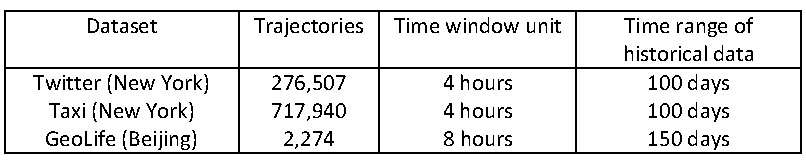
\includegraphics[width=1.0\columnwidth]{Dataset}
	\caption{Experiment environment: We use three different types of datasets. For Twitter and Taxi data, we set the same experiment environment, but for GeoLife data, we set it differently to account for the lower number of daily trajectories.}
	\label{fig:dataset}
	%\vspace{-0.7cm}
\end{figure}

We evaluate the performance of our techniques in terms of the area of each sub-space (e.g., 200m, 500m, 1km, 2km, and 4km) and the number of sectors within each sub-space (4, 6, and 8 sectors) as described in Section~\ref{sec:discretization}. 
%against varying two parameters one a time. 
%Firstly, we vary the grid size (500m, 1km, 2km, and 4km) to investigate the effect of the grid size.
%The second parameter is the number of divided sectors (4, 6, and 8 sectors) to measure the effectiveness of the number of sectors described in Section~\ref{sec:discretization}.
%To evaluate our algorithm, 
%We use two different measures: (1) Normalized Root Mean Square Error (NRMSE)~\cite{Hyndman:2006:Another}, and (2) Mean Absolute Scaled Error (MASE)~\cite{Hyndman:2006:Another}.
%We use the NRMSE measure instead of the Root Mean Square Error (RMSE) to help mitigate for the influence of outliers that generate a low reliability in the evaluation. 
We use Normalized Root Mean Square Error (NRMSE)~\cite{Hyndman:2006:Another} instead of the Root Mean Square Error (RMSE) to help mitigate for the influence of outliers that generate a low reliability in the evaluation and for scale-independent.
The measure is also widely applicable, and easily interpretable. 

%Root Mean Square Error (RMSE) is one of the most popular techniques to measure forecast accuracy~\cite{Hyndman:2006:Another} and NRMSE nomalizes the RMSE. 
%. In this work, we use a family of RMSE, different version, normalizing the RMSE, because RMSE has some drawbacks, such the high influence of outliers in the data and a low reliability.

To compute NRMSE, we first define two time series: (1) Historical time series defined by $Y_k = \left\{y_t: t \in T\right\}$, where $k = \left\{1, \cdots, S\right\}$, and (2) Forecasted time series given by ${\hat{Y}}_k = \left\{{\hat{y}}_t: t \in T\right\}$. 
NRMSE can be calculated as follows:
%In this work, we define NRMSE as
\begin{equation}
NRMSE = \frac{1}{y_{max} - y_{min}}\sqrt {{\frac{{\sum\limits_{{t = 1}}^T {{{\left( {{y_t} - {{\hat{y}}_t}} \right)}^2}} }}{{T}}}}
\end{equation}

%In our experiments, we need to compare the forecast accuracy across time series on different scales. 
%To this end, we also utilize MASE due to its scalability and applicability.  %. The major advantage of MASE is scale-independent. 
%%We first calculate the scaled errors $q_t$ that are defined as:
%The MASE error is calculated using the following equation:
%%The basis for calculating the value of the scaled errors $q_t$ is defined as: 
%\begin{equation}
%MASE = mean(|\frac{{y_t} - {{\hat{y}}_t}}{\frac{1}{T-1} \sum\limits_{{t = 2}}^T | y_t - y_{t-1}|}|)
%\end{equation}
%%The MASE error is then calculated according to:
%%\begin{equation}
%%MASE = mean(|q_t|)
%%\end{equation}
%The error is less than one if the proposed forecast method gives, on average, smaller errors than the one-step error of a naive forecast.
%Conversely, the error is greater than one, the forecasts are worse than the average one-step error.
%DOES THIS MEAN THAT WE ARE AIMING FOR MASE = 1; I.E., THIS IS THE BEST CASE SCENARIO? IF SO, THEN DRAW A THICK LINE ON 1 IN FIGURE.
%We repeat these error measurements 30~times. 
%For each trial, we forecast for different dates and compute the average of all errors.

\textbf{Varying grid sizes:} First, we show the trend in NRMSE with respect to grid sizes (granularity) in Figures~\ref{fig:Chart_NRMSE_Grid}.
For each conditions, we use a fixed number of sectors as~8. 
For GeoLife data, we cannot measure the accuracy when the grid size is less than 500 meters, because of many data sparsity issues in sub-spaces that have no trajectories.
For the Twitter and the Taxi data that have a relatively high trajectory density, we find that both errors increase as the grid size grows.
This shows that a larger area can have high directional uncertainty in forecasting human mobility.
In contrast, for the GeoLife data, the error significantly decreases because the sparsity decreases as the grid size increases.
%For MASE, the size of grid has little effect on the forecast accuracy for the Twitter and Taxi data.
%However, for the GeoLife data, it has a large impact on forecasting accuracy, but the accuracy for the data is still low.
%WHAT DOES THIS TELL ME?? WHAT CONCLUSIONS CAN WE MAKE?
We discuss these results further in Section~\ref{sec:discussion}.

\textbf{Varying sector numbers:} Next, we investigate the effect of the number of sectors on the performance of our technique.
We perform an experiment with three different conditions: 4, 6, and 8 sectors with a fixed grid size of 1~km.
For example, for each sub-space, if we divide one full turn (360\degree) into 4~circular sectors of the same size, each sector will cover 90\degree.
By varying the number of sectors, the NRMSE measure show the forecasting accuracy increase as the number of sectors grows as shown in Figure~\ref{fig:Chart_NRMSE_Sector}.
It proves that our algorithm successfully improve the forecast performance.
%we little impact is observed for forecasting accuracy of the Twitter and Taxi datasets as shown in Figure~\ref{fig:Chart_NRMSE_Sector}.
However, for GeoLife data, the measure shows the error rate increases as the number of sectors grows.
%WHAT DOES THIS SHOW? NEED TO MAKE SOME OBSERVATIONS HERE. 
These results are discussed further in Section~\ref{sec:discussion}.


%\begin{figure}[tbh]
	%\centering
	%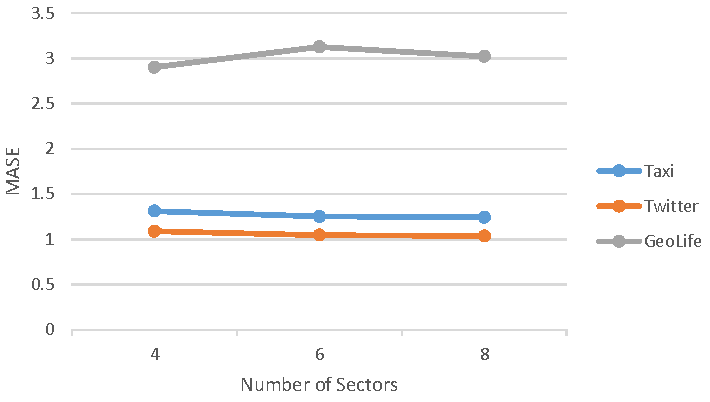
\includegraphics[width=1.0\columnwidth]{Chart_MASE_Sector}
	%\caption{MASE vs the number of sectors}
	%\label{fig:Chart_MASE_Sector}
%\end{figure}


%\begin{figure*}[tbh]
	%\centering
	%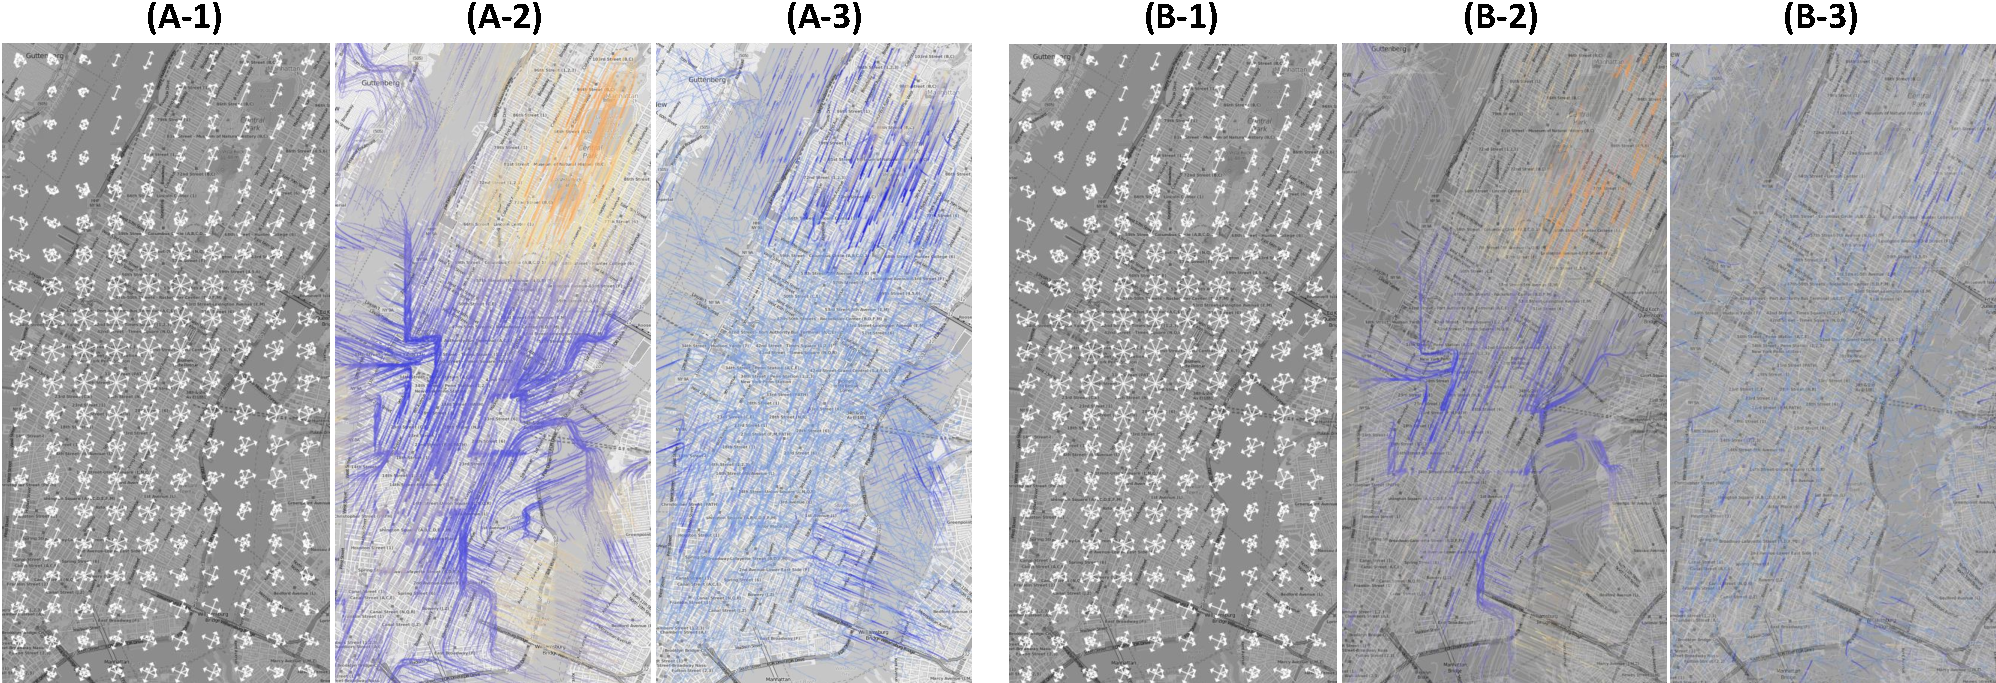
\includegraphics[width=1.0\linewidth]{nyc_forecasting_result}
	%\caption{An example of forecasting result. (A-1) Observed directional density (A-2) Observed major flows (A-3) Observed other flows (B-1) Forecasted directional density (B-2) Forecasted major flows (B-3) Forecasted other flows}
	%\label{fig:forecasting_result}
	%%\vspace{-0.7cm}
%\end{figure*} 